\documentclass[aspectratio=169]{beamer}

\setbeameroption{show notes on second screen}

\usepackage[utf8]{inputenc}
\usetheme{Madrid}
\usecolortheme{beaver}

\usepackage{graphicx}
\graphicspath{ {../Resources/} }

\title{Critical Design Review}       % Title
\author{Austin, Joe, Matt, Kathryn}                     % Team members
\institute{SNHU/CETA}                                   % Institute
\logo{
\includegraphics[height=0.8cm]{../../AJMK_Logo}}  % Our Logo
\titlegraphic{
\includegraphics[height=2.6cm]{Stencil.png}} % Title graphic

\begin{document}

\frame{\titlepage} % Draw the title page
\note{Title page notes here.}

\section{Introduction}

\begin{frame}
    \frametitle{Agenda}

    \begin{columns}
    \begin{column}{0.48\textwidth}
        \setcounter{tocdepth}{1} % Prof requested we do this
        {\tableofcontents}
    \end{column}

    \begin{column}{0.48\textwidth}
        \begin{center}
            
\includegraphics[height=3cm]{../../AJMK_Logo}
            
\includegraphics[height=3cm]{Stencil.png}
        \end{center}
    \end{column}
    \end{columns}

\note{
\huge Everyone \normalsize

\begin{itemize}
 \item We'll do questions at the end
 \item Page numbers are in the bottom right, remember to note what page you'd like us to go back to!
\end{itemize}
}
\end{frame}

\section{ConOps Summary}
\begin{frame}
    \frametitle{ConOps Summary}

    \begin{columns}

    \begin{column}{0.34\textwidth}
        Stakeholders
        \begin{itemize}
         \item SNHU
         \item Professors
         \item Industrial Trainers
         \item Parts and manufacturers
        \end{itemize}

        Users
        \begin{itemize}
         \item Pendulum Team
         \item Educators
        \end{itemize}
    \end{column}

    \begin{column}{0.65\textwidth}
        \begin{block}{Operating Modes}
            \begin{enumerate}
            \item Off mode
            \item Idle mode
            \item Spinup mode
            \item Demo mode
            \item User PID mode
            \end{enumerate}
        \end{block}

        \begin{block}{System Description}
            \small{An inverted pendulum is a type of PID Demonstrator, where a simple PID loop
            controls and minimizes the error in a system, in this case, the error is the angle of the pendulum. A perfectly tuned PID loop will hover the pendulum.}
            \textbf{Perfectly Still}.
        \end{block}
    \end{column}
\end{columns}

\note{
\huge Matt \normalsize

\begin{itemize}
 \item So our stakeholders include SNHU, our professors, industrial trainers and of course the people who supply parts and manfucacture our product.
 \item At the moment, we're the ones manufacturing it but in the future it could be different.
 \item Our users are us and educators who might want to use this product to teach the fundamnetals of PID
 \item It has a few modes, Off, Idle, Spinup, Demo and user PID mode. The last two are where the pendulum self-balances
 \item Its almost like a game, the system is naturally unstable, the pendulum wants to fall, but a properly tuned PID loop can keep it upright!
\end{itemize}
}

\end{frame}

\begin{frame}
    \frametitle{ConOps (cont.)}

    \begin{columns}
        \begin{column}{0.48\textwidth}
            \begin{block}{Operation and Support Environment}
                \begin{itemize}
                 \item Built from COTS (common off the shelf) parts
                 \item Designed to be serviced
                 \item Constant Uptime
                 \item Low power modes
                \end{itemize}
            \end{block}
        \end{column}

        \begin{column}{0.48\textwidth}
            \begin{block}{Impact considerations}
                \begin{itemize}
                 \item Requiring physical space, either for storage or use.
                 \item Being a hazard and risking misuse.
                 \item Generating pollutants and disposal.
                \end{itemize}
            \end{block}
        \end{column}
    \end{columns}

\note{
\huge Matt \normalsize

\begin{itemize}
 \item Being built from COTS parts allows us to easily replace components and design service schedules
 \item We also have plans for a low power mode and folding or removable legs to decrease electrical and physical footprint.
\end{itemize}
}

\end{frame}

\section{Studies}
\begin{frame}
    \frametitle{Summary of Trade Studies}

    \begin{columns}
        \begin{column}{0.70\textwidth}
            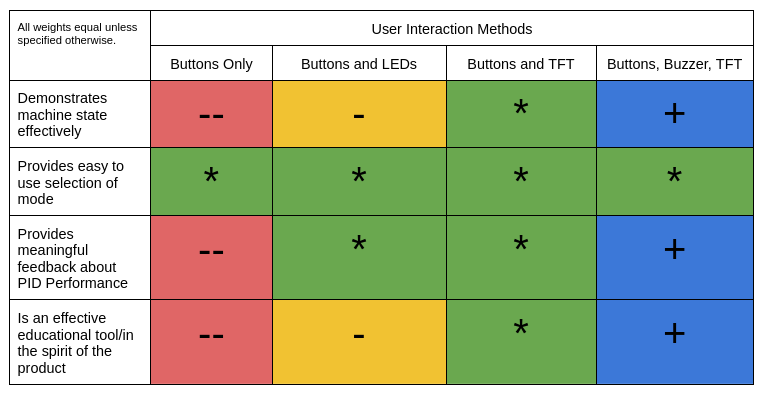
\includegraphics[width=10.5cm]{UserInteractionTradeStudy}
        \end{column}

        \begin{column}{0.28\textwidth}
            \begin{block}{User Interactions}
                The way the user interacts with our system is an important
                part of our design, if the system does not meaningfully
                interact with the operator, than it does not perform
                to our requirements.
            \end{block}
        \end{column}
    \end{columns}

    \note{
        Notes here
    }
\end{frame}

\begin{frame}
    \frametitle{Summary of Trade Studies (cont.)}

    \begin{columns}
        \begin{column}{0.28\textwidth}
            \begin{block}{Bearings}
                Choosing bearings that meet our minimum requirements
                helps us to design a system that meets the needs we
                expect to solve.
            \end{block}
        \end{column}

        \begin{column}{0.70\textwidth}
            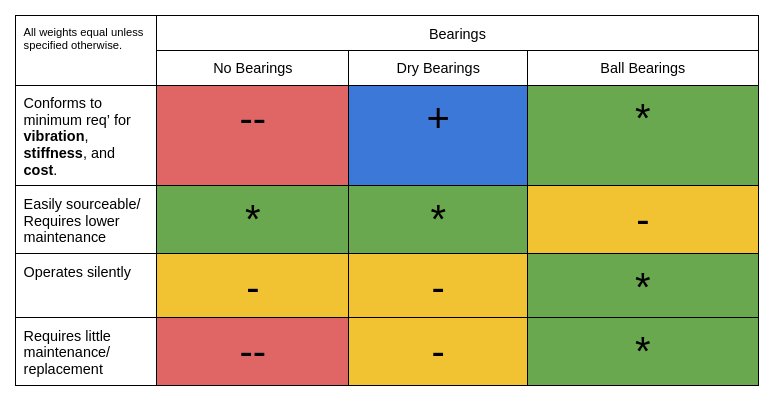
\includegraphics[width=10.5cm]{BearingsTradeStudy}
        \end{column}
    \end{columns}

    \note{
        Notes here
    }
\end{frame}

\begin{frame}
    \frametitle{Summary of Trade Studies (cont.)}

    \begin{columns}
        \begin{column}{0.70\textwidth}
            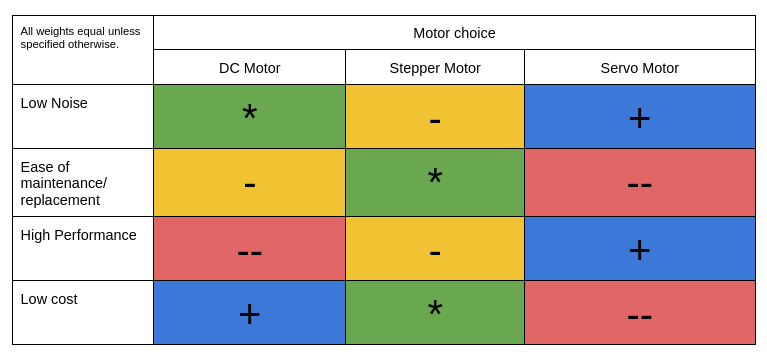
\includegraphics[width=10.5cm]{MotorTradeStudy}
        \end{column}

        \begin{column}{0.28\textwidth}
            \begin{block}{Motors}
                We use our requirements to balance weight, sound
                cost and performance.
            \end{block}
        \end{column}
    \end{columns}

    \note{
        Notes here
    }
\end{frame}

\begin{frame}
    \frametitle{Summary of Trade Studies (cont.)}

    \begin{columns}
        \begin{column}{0.28\textwidth}
            \begin{block}{Material Choice}
                Different Materials lol
            \end{block}
        \end{column}

        \begin{column}{0.70\textwidth}
            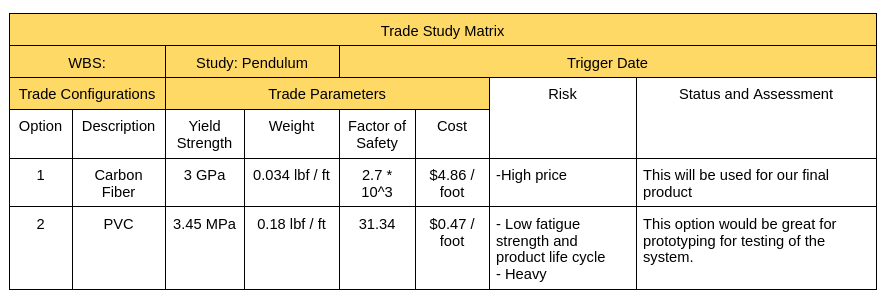
\includegraphics[width=10.5cm]{MaterialTradeStudy}
        \end{column}
    \end{columns}

    \note{
        Notes here
    }
\end{frame}

\begin{frame}
    \frametitle{Summary of Trade Studies (cont.)}

    \begin{columns}
        \begin{column}{0.70\textwidth}
            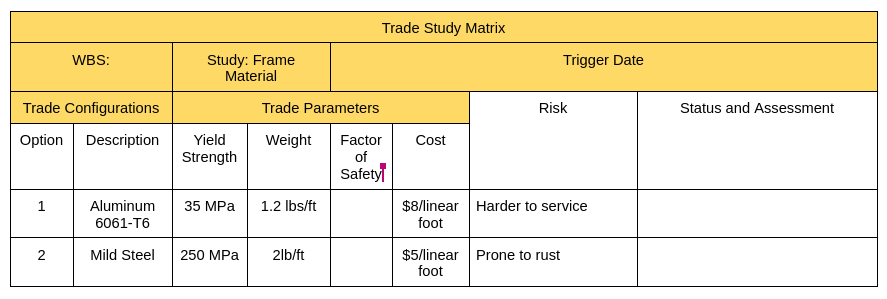
\includegraphics[width=10.5cm]{MetalTradeStudy}
        \end{column}

        \begin{column}{0.28\textwidth}
            \begin{block}{Metal}
                The metal we select affects safety and cost.
            \end{block}
        \end{column}
    \end{columns}

    \note{
        Notes here
    }
\end{frame}

\begin{frame}
    \frametitle{Summary of Trade Studies (cont.)}

    \begin{columns}
        \begin{column}{0.28\textwidth}
            \begin{block}{NEMA Motor Choice}
                The specific type of stepper motor impacts strngth and idle power.
            \end{block}
        \end{column}

        \begin{column}{0.70\textwidth}
            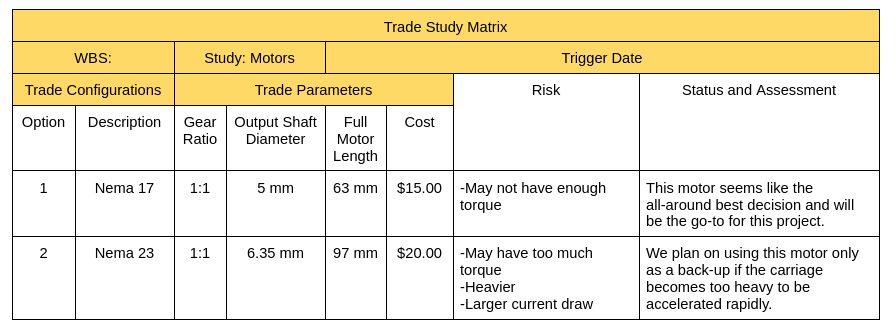
\includegraphics[width=10.5cm]{MotorTradeStudy2}
        \end{column}
    \end{columns}

    \note{
        Notes here
    }
\end{frame}

\section{Requirements}
\begin{frame}
    \frametitle{Functional Requirements}

    \begin{columns}
        \begin{column}{0.70\textwidth}
            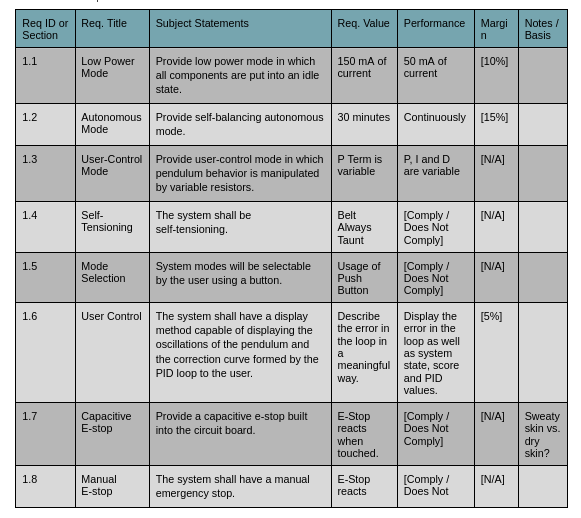
\includegraphics[height=7cm]{Functional1}
        \end{column}

        \begin{column}{0.28\textwidth}
            \begin{block}{Functional Requirements}
                MISSING\_TEXT
            \end{block}
        \end{column}
    \end{columns}

    \note{
        Notes here
    }
\end{frame}

\begin{frame}
    \frametitle{Functional Requirements (cont.)}

    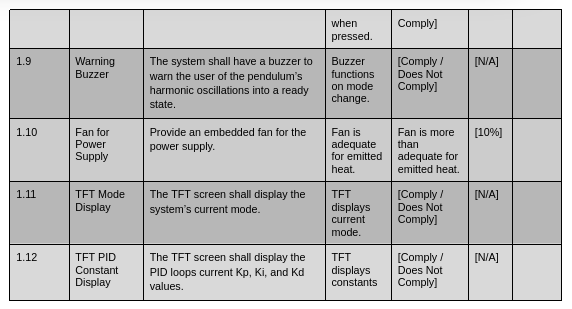
\includegraphics[height=7cm]{Functional2}
\end{frame}

\begin{frame}
    \frametitle{Performance Requirements}

    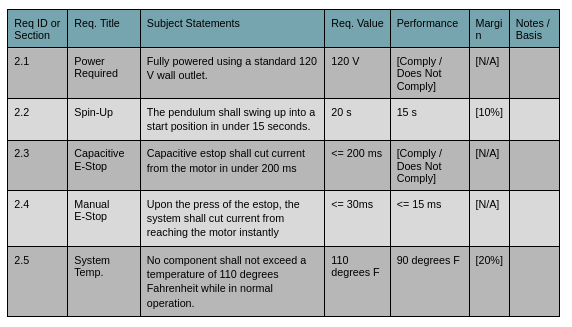
\includegraphics[height=7cm]{Performance}
\end{frame}


\begin{frame}
    \frametitle{Other Requirements}

    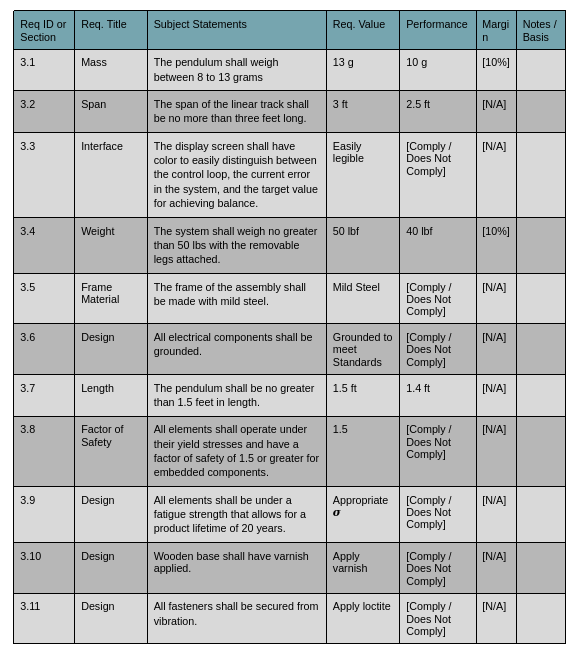
\includegraphics[height=7cm]{OtherReqs}
\end{frame}


\section{Design}
\begin{frame}
    \frametitle{System Design}

    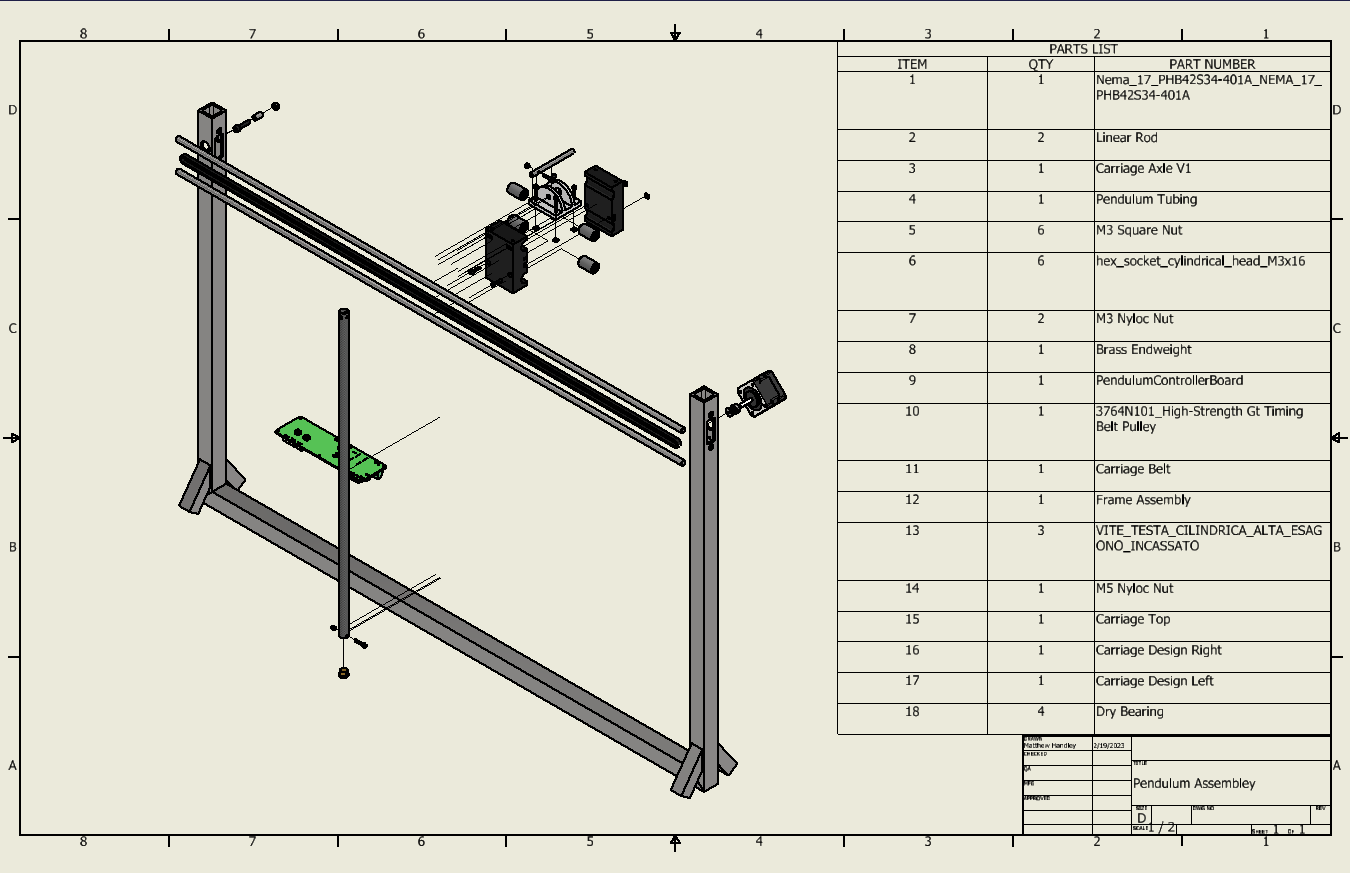
\includegraphics[width=10.5cm]{exploded}

    \note{
        Done by matt

        Note that the tubing contains all cutouts and motor mounts, eliminating
        the need for expensive dedicated brackets and fixtures.
    }
\end{frame}

\begin{frame}
    \frametitle{Bill Of Materials}

    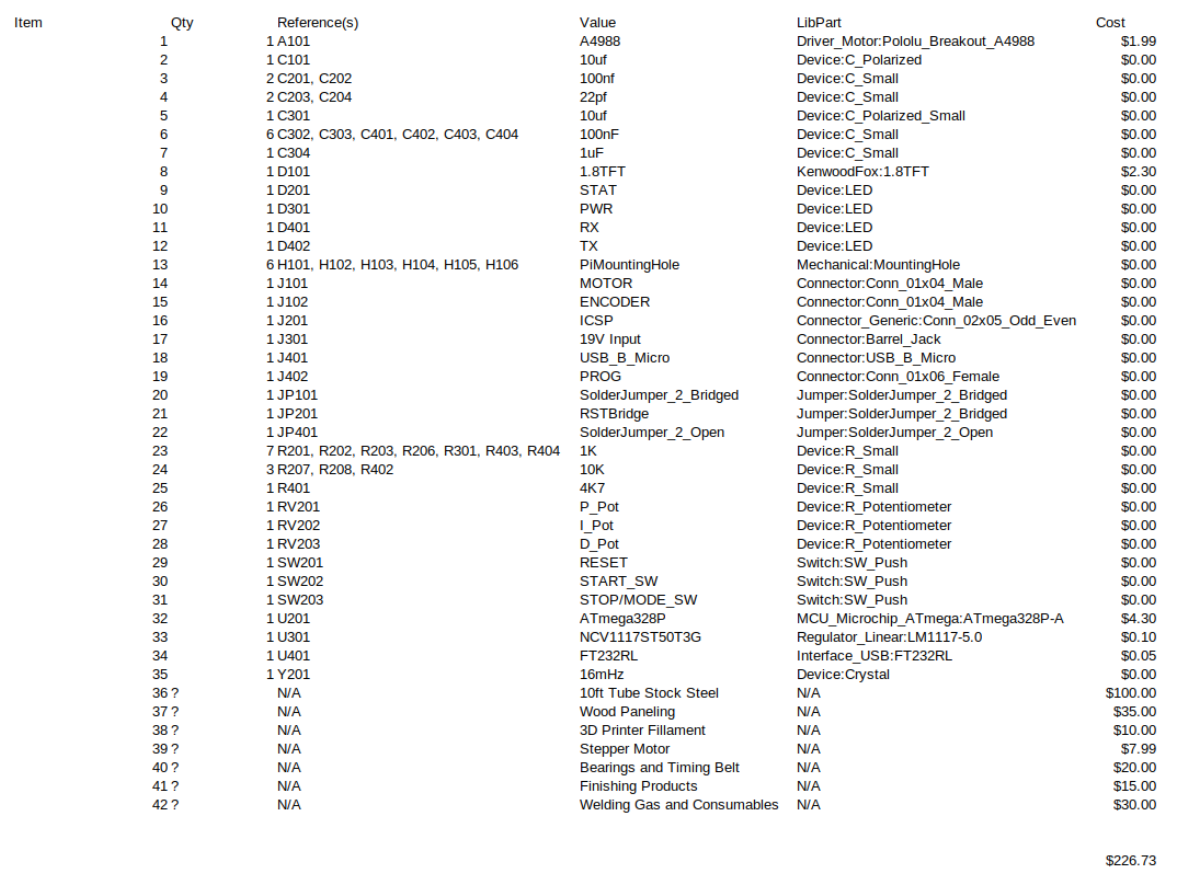
\includegraphics[height=7cm]{BOMTable}

    \note{
        Our bill of materials is very long but everything is here even down
        to the smallest individual components.
    }
\end{frame}

\begin{frame}
    \frametitle{Ordering Status}

    \begin{block}{Bearings}
        Both dry and ball bearings have been ordered.
    \end{block}

    \begin{block}{PCB}
        We've submitted our PCB but have not yet confirmed order.
    \end{block}

    \begin{block}{Steel}
        We're in the process of sourcing steel.
    \end{block}

    \begin{block}{3D/plastic/COTS}
        Material stock for welding, 3D printing and machining are ready to go.
    \end{block}
\end{frame}


\begin{frame}
    \frametitle{Safety}

    \begin{columns}
        \begin{column}{0.75\textwidth}
            \begin{block}{Our Safety Statement}
                One concern for public health in our design is the swinging pendulum itself which can hit and hurt someone if not used properly or tamper with the safety mechanisms in place on the system. The safety mechanism in place is a hard stop button if the system malfunctions. It serves to stop the system cold as well as a mechanism to detect if the pendulum hits something such that it will stop the system as well. In addition to those we plan to implement a screen between the user and the swinging pendulum. Another concern is the electronics inside overheating and causing fire. This is presented by the operation conditions to be placed in a lab room. To combat this the system has very low voltage running it such that overheating causing damage or fire is unlikely even with constant use.
            \end{block}
        \end{column}

        \begin{column}{0.20\textwidth}
            We know our product presents some safety concerns. We've developed
            requirements for safe operation such as \textbf{shields} and
            \textbf{software limits}.
        \end{column}
    \end{columns}

    \note{
        Shields, software limits, and our overall design philosophy drives
        a safe system.
    }
\end{frame}


\begin{frame}
    \frametitle{Impact Considerations}

    \begin{enumerate}
        \item Being a hazard and risking misuse.
        \item Requiring physical space, either for storage or use.
        \item The system will generate waste at the end of its life cycle. The goal is to minimize this waste through the use of recyclable materials
    \end{enumerate}

    \note{
        Notes here
    }
\end{frame}

\section{Calibration and Maintenance}
\begin{frame}
    \frametitle{Calibration and Maintenance}

    \begin{enumerate}
        \item The system shall perform a self-test on start-up. Due to the pendulum hanging towards the center of the earth due to gravity, the encoder on the pendulum will be zeroed using the position.
        \item The motor shall move towards a limit switch at a set slow speed until it triggers one of the two limit switches on either side of the linear rails, upon triggering one, the carriage will then move a set amount of motor steps to the middle of the span of the linear rails.
        \item All fasteners shall have their tightness ensured before operation, and any renewal of lubrical for the pendulum shall be performed.
        \item A maintenance and component replacement manual shall be created in order to easily explain how to replace the COTS (common of the shelf) parts such as the precision belt or the motor internals.
    \end{enumerate}

    \note{
        Notes here
    }
\end{frame}

\section{Subsystems}
\begin{frame}
    \frametitle{The Mechanical Subsystem}

    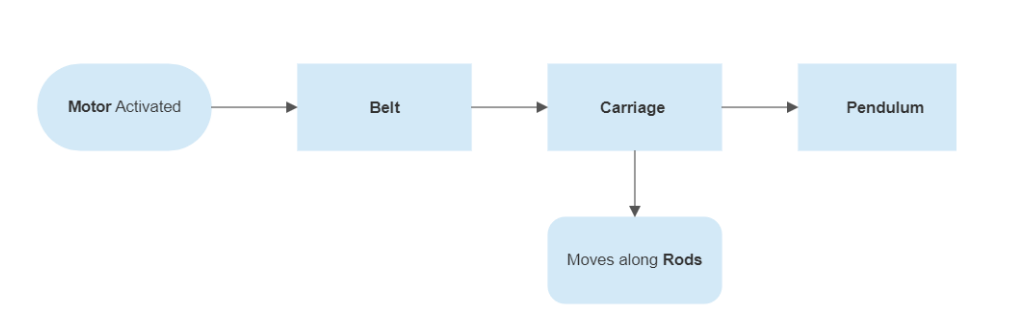
\includegraphics[width=15cm]{MechanicalSubsystem}

    \note{
        Thank you austin!
    }
\end{frame}

\begin{frame}
    \frametitle{The Software/Electrical Subsystem}

    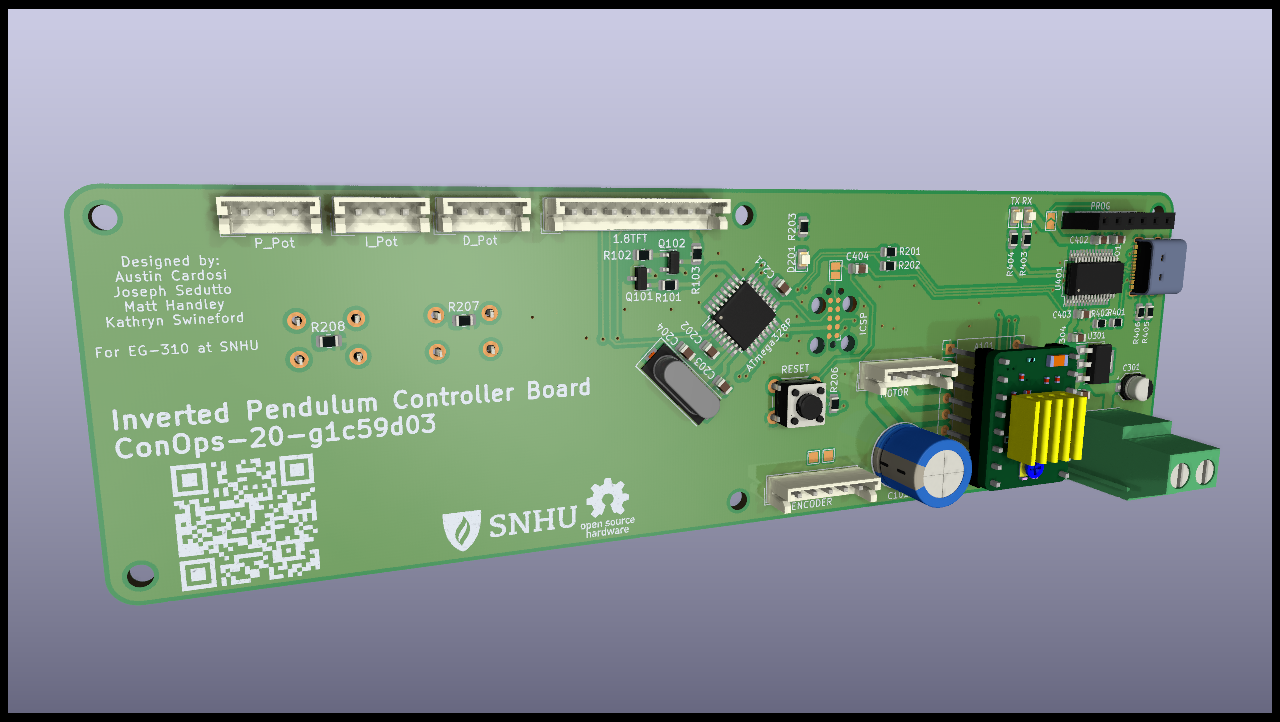
\includegraphics[height=7cm]{CircuitBoard}

    \note{
        In our system the software and hardware are very closely
        linked.

        We have several features such as the E-Stop that
        rely heavily on an integration between embedded code
        and physical electrical hardware interlocks.
    }
\end{frame}

\begin{frame}
    \frametitle{The Software/Electrical Subsystem (cont.)}

    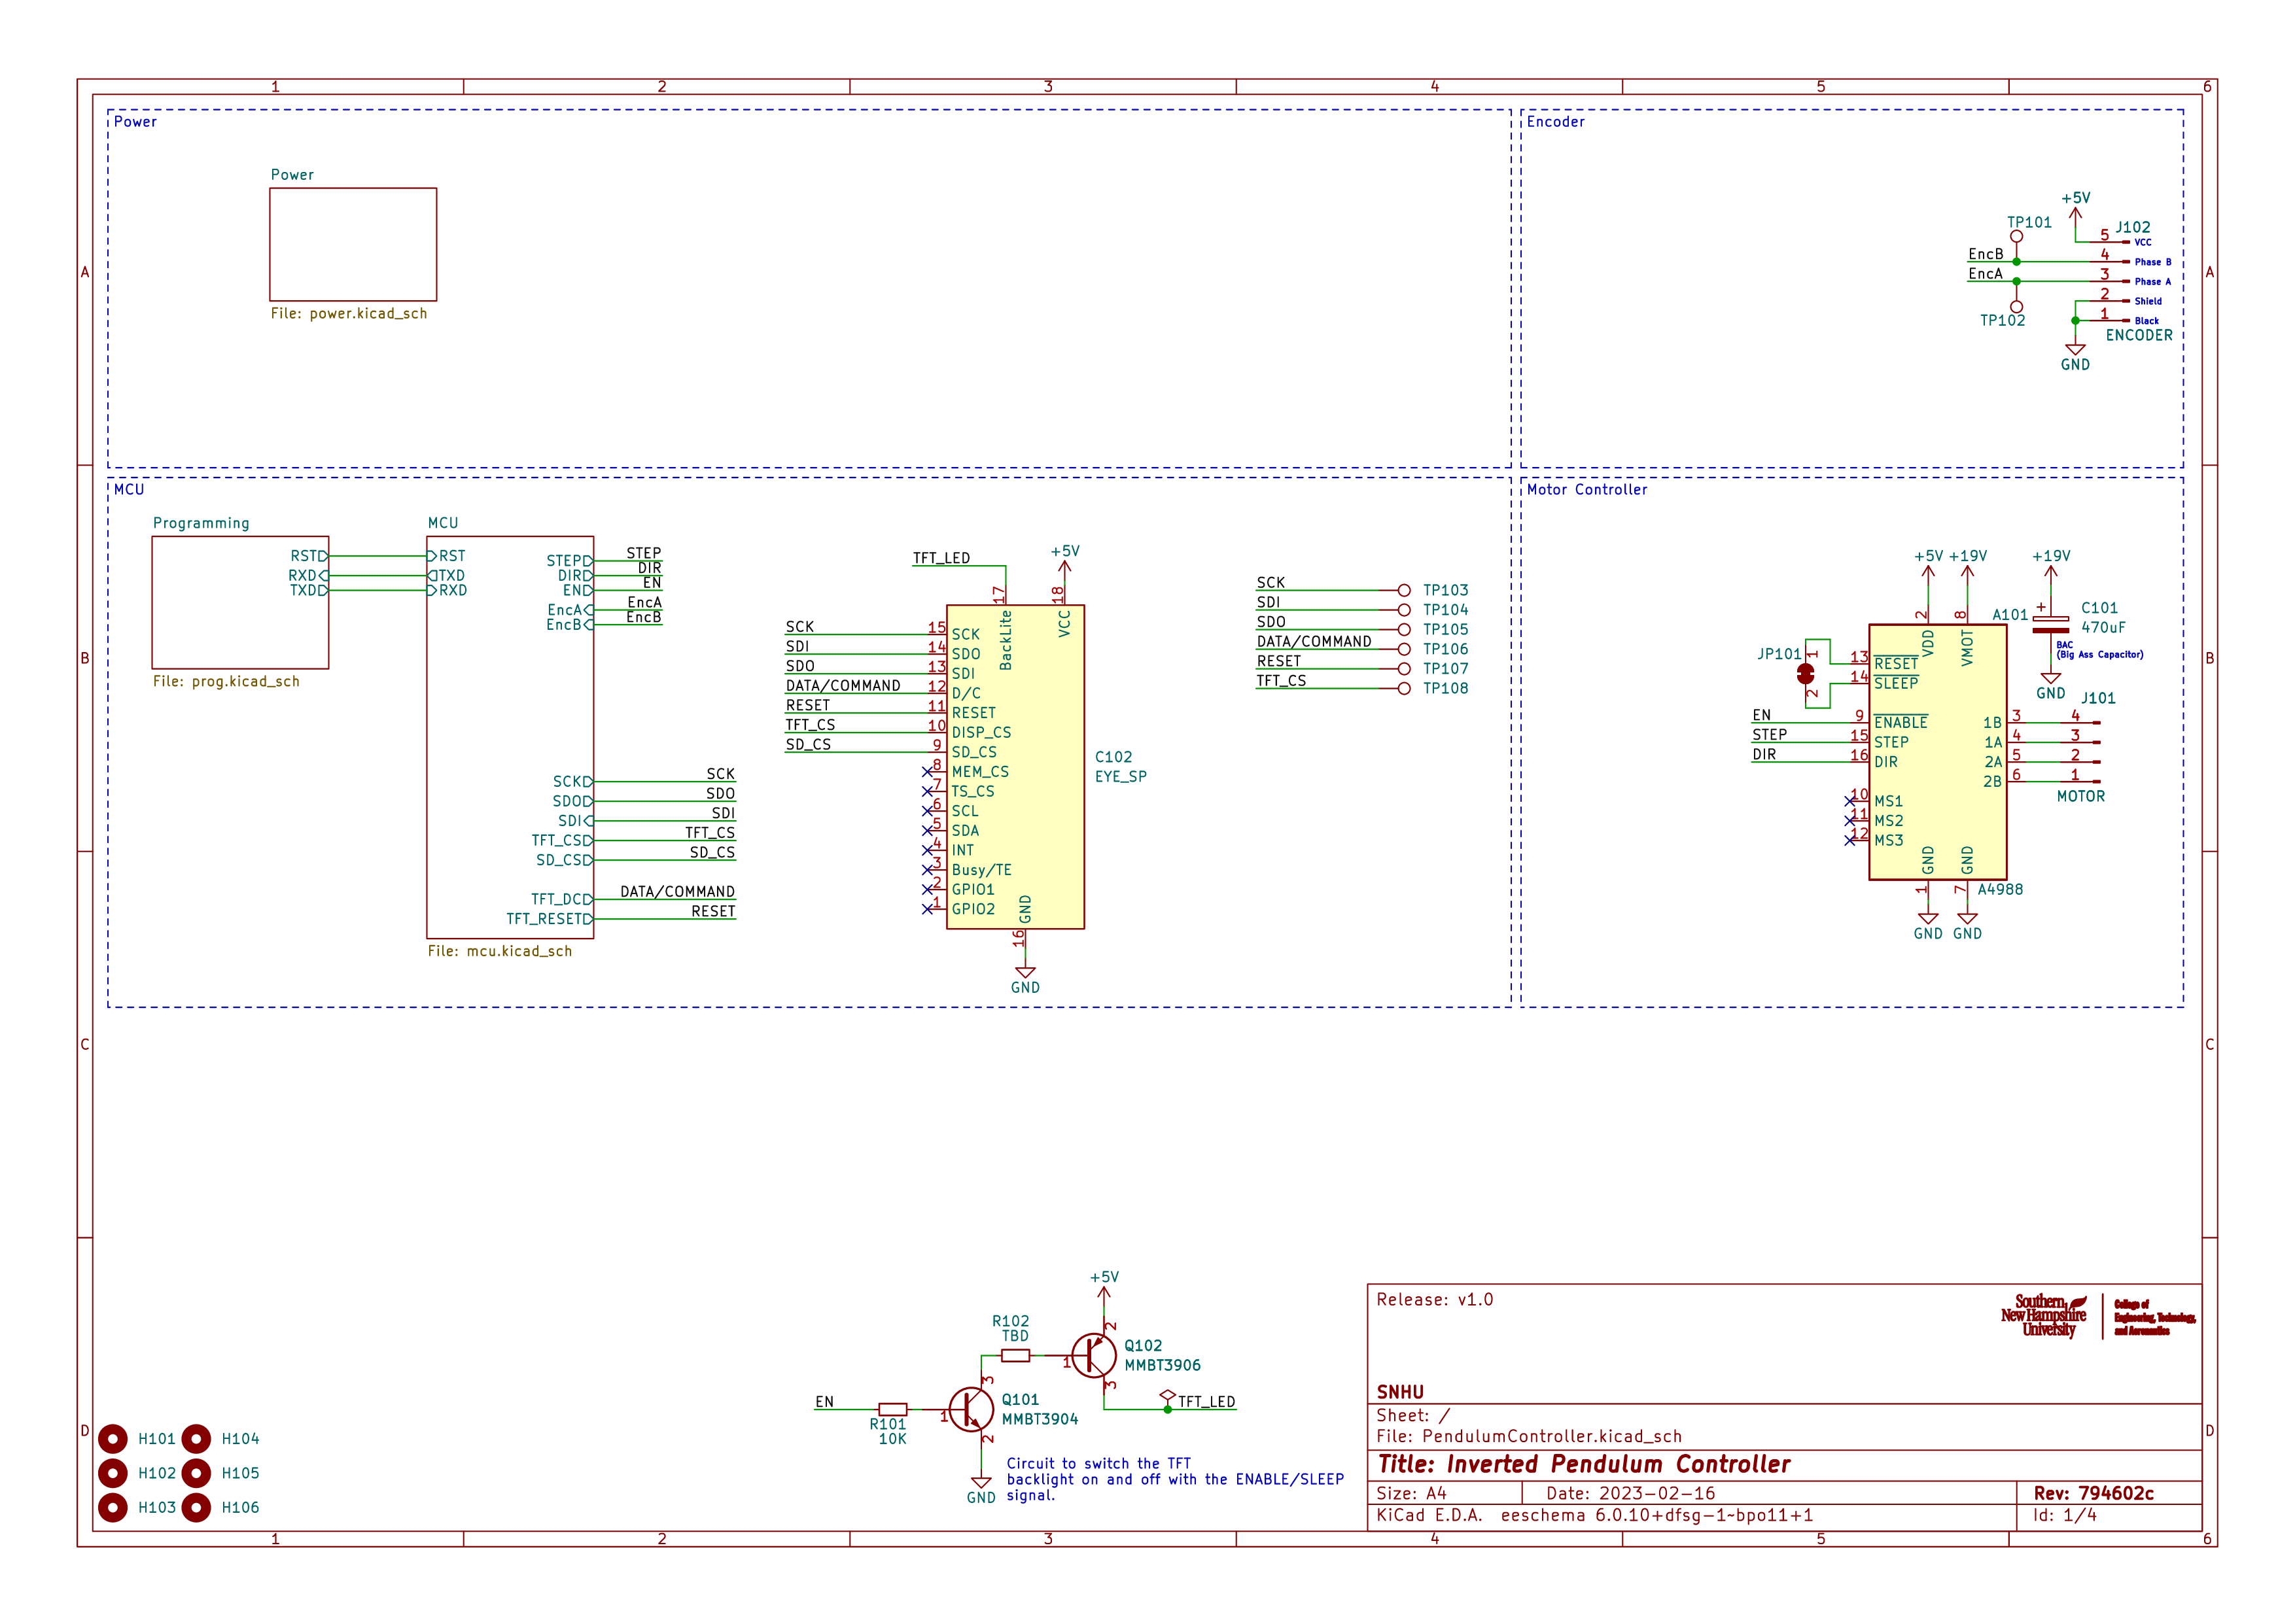
\includegraphics[height=7cm]{Schematic}

    \note{
        We've designed the general circuitry to take advantage of every
        safety feature the 328p offers such as:
        \begin{enumerate}
         \item A hardware watchdog
         \item Integrated current monitoring
         \item A standby shutdown
         \item And an integrated clock
        \end{enumerate}

    }
\end{frame}

\begin{frame}
    \frametitle{Safety}

    Health and Safety Design Features:
    \begin{enumerate}
        \item Protective shielding around the pendulum’s range of motion to avoid pinch points and physical contact.
        \item Capacitive e-stop and manual e-stop in case of emergency.
        \item All electrical components are grounded to prevent dangerous discharge.
        \item All components shall be ventilated and fan cooled to regulate temperatures.
        \item Access to embedded components shall be easy to clean the machine and remove dust and debris.
    \end{enumerate}

    \note{
        Most important features are sheilding

        capactive estop

        grounding

        access to cleaning to remove dust and prevent overheating
    }
\end{frame}

\section{CDR Specifics}
\begin{frame}
    \frametitle{Verification Plan (Electrical/Software)}

    \begin{columns}
        \begin{column}{0.58\textwidth}
            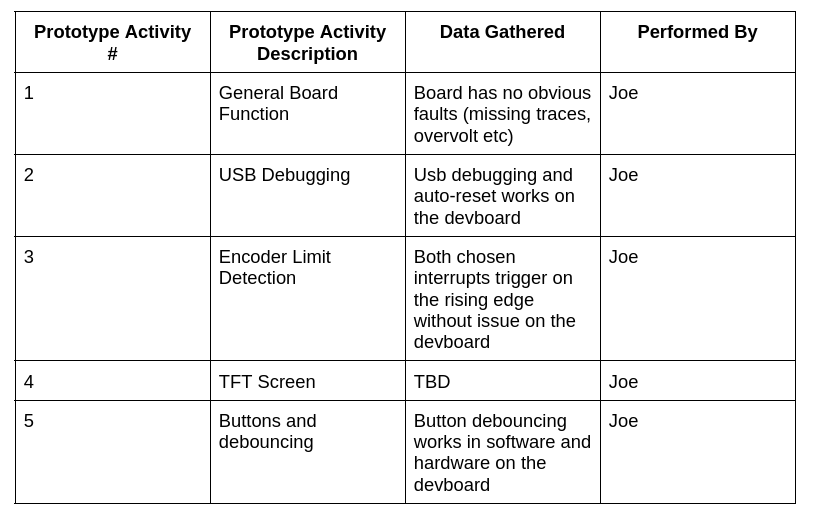
\includegraphics[width=8.5cm]{ElectricalPrototype}
        \end{column}

        \begin{column}{0.40\textwidth}
            \begin{block}{Block Diagram}
                \tiny{
                    Mainboard requires several important features:
                    \begin{enumerate}
                        \item E-Stop
                        \item Button Inputs
                        \item Potentiometers
                        \item Encoder
                        \item Motor output
                        \item Limit Switch
                        \item TFT Screen
                    \end{enumerate}

                    The prototype board implements all these features as well as...
                    \begin{enumerate}
                        \item USB Programming/debugging
                        \item Status lights
                        \item Mode and start select buttons
                        \item Onboard VRM
                    \end{enumerate}
                }
            \end{block}
        \end{column}
    \end{columns}

    \note{
        The electrical components must adheere to the standards we set
        and must pass our tests

        The most important tests are that the board \textbf{Generally Functions}
        and that we can \textbf{Program and Debug} it without an external
        programmer.
    }
\end{frame}

\begin{frame}
    \frametitle{Verification Plan (Mechanical)}

    \begin{columns}
        \begin{column}{0.40\textwidth}
            \begin{block}{Block Diagram}
                \tiny{
                    Each bearing is tested and evaluated with the above chart, with specific attention to:
                    \begin{enumerate}
                        \item Cost of bearing (4 needed for every pendulum)
                        \item Noise (Minimize sliding grinding noises)
                        \item Performance (How well does it slide and protect the carriage shafts)
                        \item Longevity (How long does it last without service or lube?)
                    \end{enumerate}
                }
            \end{block}
        \end{column}

        \begin{column}{0.58\textwidth}
            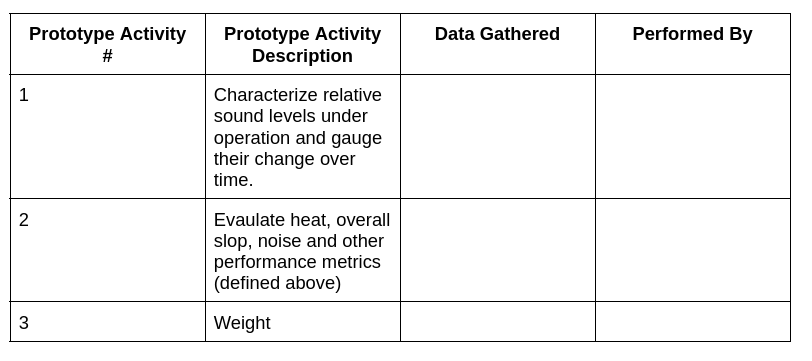
\includegraphics[width=8.5cm]{MechanicalPrototype}
        \end{column}
    \end{columns}

    \note{
        Might need matt input
    }
\end{frame}


\begin{frame}
    \frametitle{Phase D}

    \begin{enumerate}
        \item All drawings and assemblies are on the latest revision and meet all specifications
        \item All required parts will be ordered through Carlstrom / Joe Donovan this week (2/22/2023)
        \item Manufacturing of the frame will begin as soon as the steel is delivered, and prototyping of parts will begin once all remaining parts are delivered.
        \item Drawings and assemblies will be finalized this weekend (2/25/2023 for machining to begin.
    \end{enumerate}


    \note{
        Notes here
    }
\end{frame}


\section{Diagrams}
\subsection{Block Diagrams}
\begin{frame}
    \frametitle{Block Diagram}

    \begin{columns}
        \begin{column}{0.70\textwidth}
            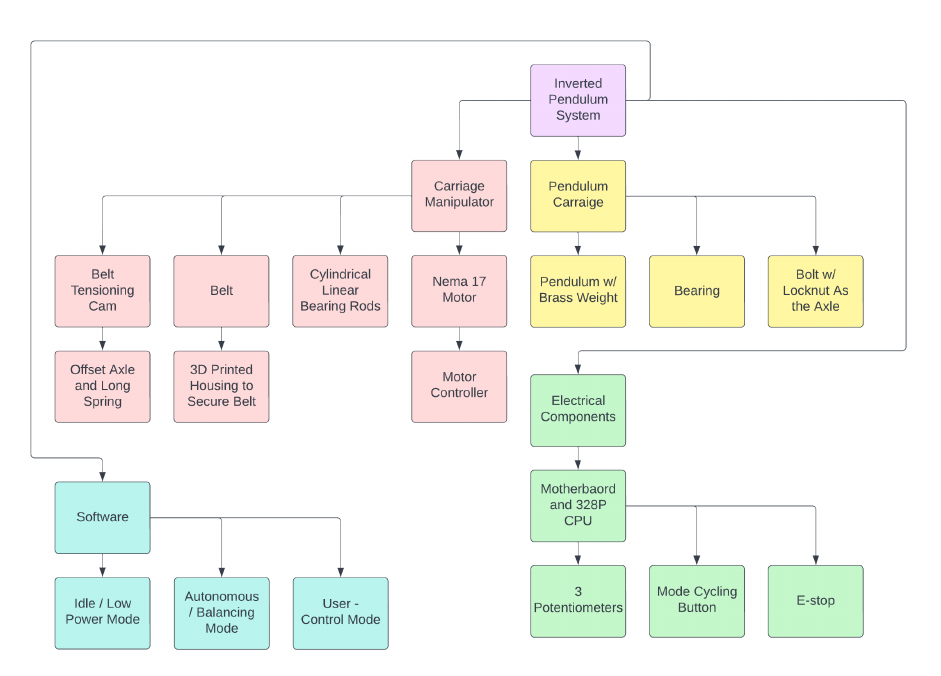
\includegraphics[height=7cm]{BlockDiagram}
        \end{column}

        \begin{column}{0.30\textwidth}
            \begin{block}{Block Diagram}
                The block diagram details the electrical, mechanical and software components.
                And their relationship to each other.
            \end{block}
        \end{column}
    \end{columns}

\note{
\huge Matt \normalsize

\begin{itemize}
 \item Our block diagram shows how our software, hardware and electronics may interact in a final system
\end{itemize}
}

\end{frame}

\subsection{Operations}
\begin{frame}
    \frametitle{Operations}

    \begin{columns}
        \begin{column}{0.30\textwidth}
            \begin{block}{Operations}
                The Operations diagram details the physical and general controls.
            \end{block}
        \end{column}

        \begin{column}{0.70\textwidth}
            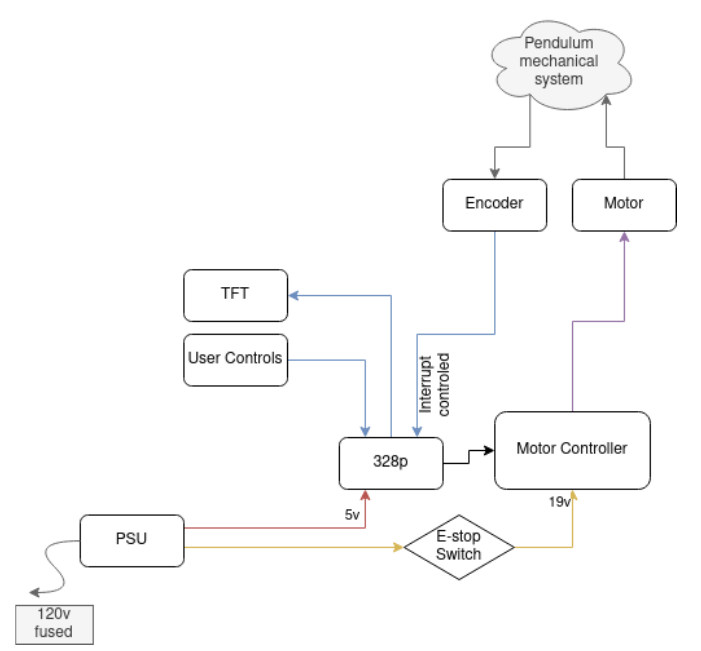
\includegraphics[height=7cm]{Operations}
        \end{column}
    \end{columns}

\note{
\huge Joe \normalsize

\begin{itemize}
 \item The operations chart details our physical and general controls like the tft screen
 \item the buttons
 \item the motor controller and encoders
\end{itemize}
}

\end{frame}

\subsection{Software}
\begin{frame}
    \frametitle{Software Flowchart}

    \begin{columns}
        \begin{column}{0.72\textwidth}
            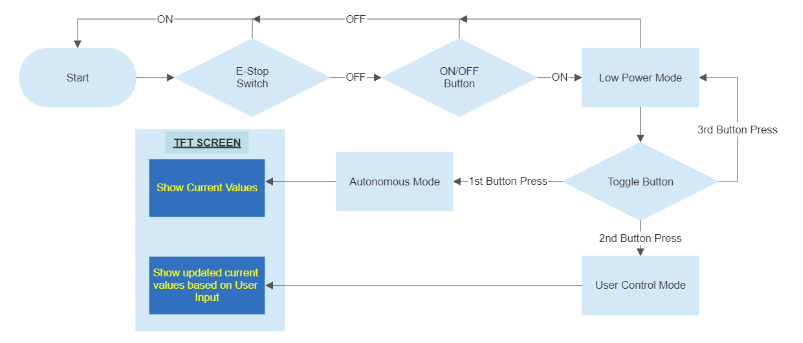
\includegraphics[width=11cm]{Operation}
        \end{column}

        \begin{column}{0.28\textwidth}
            \begin{block}{Software Flowchart}
                The software flowchart is an overview of all the software functions of our
                proposed product.
            \end{block}
        \end{column}
    \end{columns}

\note{
\huge Austin \normalsize

\begin{itemize}
 \item Our software flowchart details how the PID control scheme will be interactable by the users
\end{itemize}
}

\end{frame}


\section{End}
\begin{frame}
    \frametitle{End}

    \begin{block}{}
        \begin{center}
            \Huge Questions and Comments?
        \end{center}
    \end{block}

    \begin{center}
        Find the source code for this document, and the rest of our designs, firmware, hardware
        and notes on GitHub!

        
\includegraphics[height=2cm]{github_qr}
    \end{center}

\note{
\begin{itemize}
 \item So please if you have any questions we would love to hear them.
 \item All of our software, CAD, hardware and design docs are licensed under
 \item \huge The MIT Open Source License \normalsize and available via git.
 \item If you have a specific slide in mind we can go back to it!
\end{itemize}
}
\end{frame}

\section{Extras}
\begin{frame}
    \frametitle{Code}

    \begin{columns}
        \begin{column}{0.58\textwidth}
            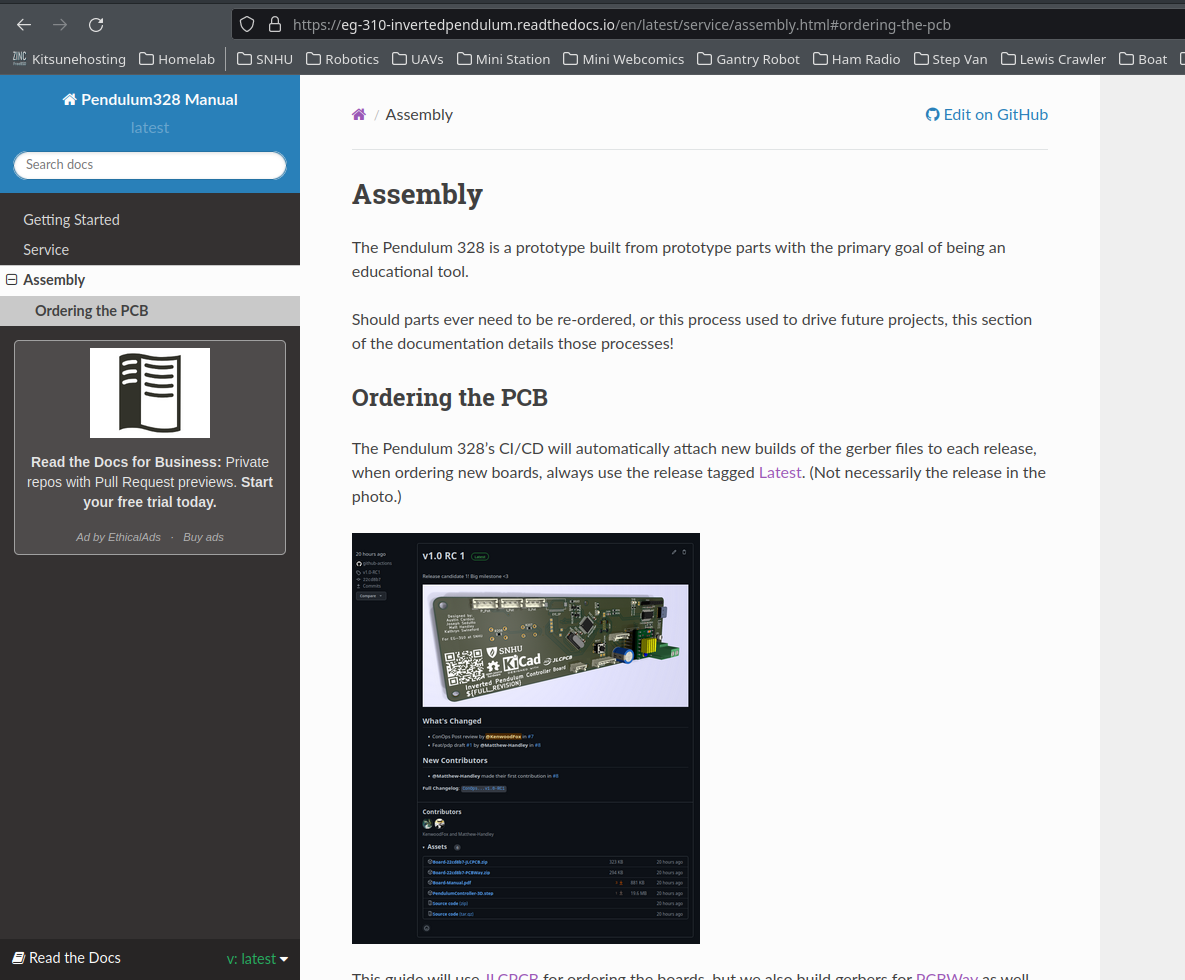
\includegraphics[height=7cm]{ManualOnline}
        \end{column}

        \begin{column}{0.38\textwidth}
            \begin{block}{Our Documentation}
                Find our docs online, built from the very code and CAD that
                makes our project, conforming closely to industry standards
                for industrial automation.
            \end{block}
        \end{column}
    \end{columns}
\end{frame}

\begin{frame}
    \frametitle{Carriage}

    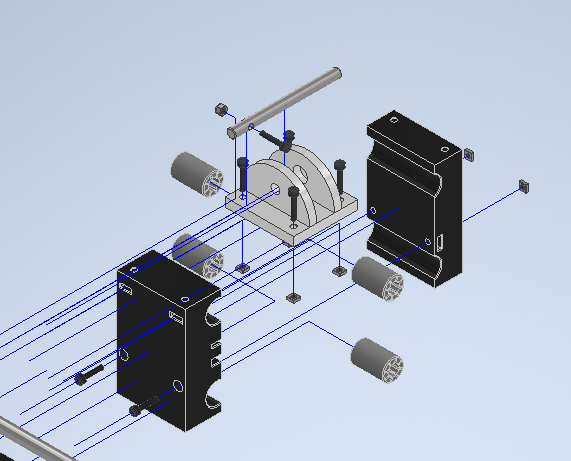
\includegraphics[height=7cm]{closeup1}
\end{frame}

\begin{frame}
    \frametitle{Carriage (cont.)}

    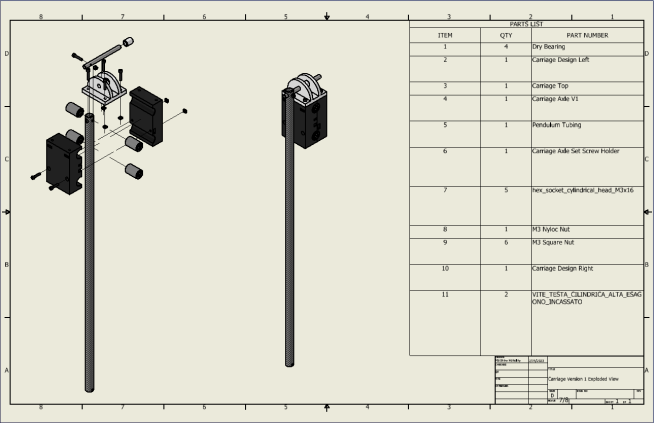
\includegraphics[height=7cm]{closeup2}
\end{frame}

\begin{frame}
    \frametitle{End Section}

    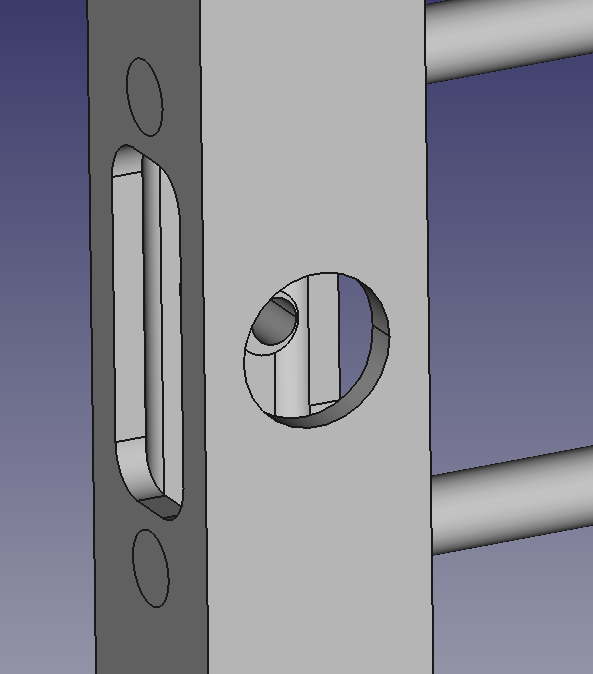
\includegraphics[height=7cm]{closeup3}
\end{frame}

\begin{frame}
    \frametitle{Bezel}

    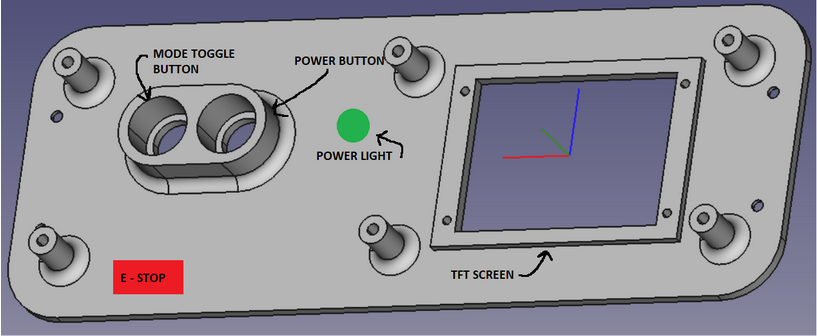
\includegraphics[height=6cm]{closeup4}
\end{frame}

\begin{frame}
    \frametitle{Carriage Render}

    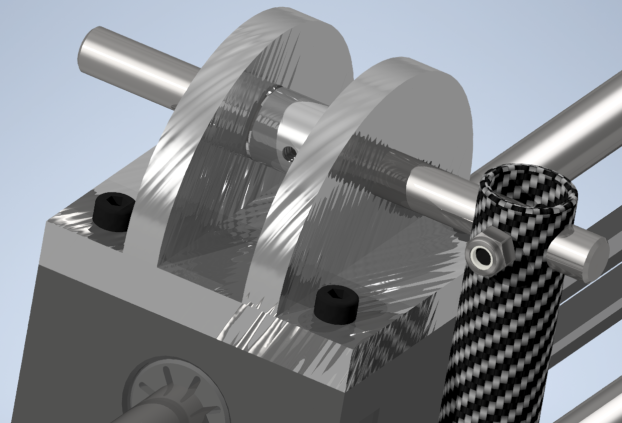
\includegraphics[height=6cm]{closeup5}
\end{frame}

\begin{frame}
    \frametitle{Calculations}

    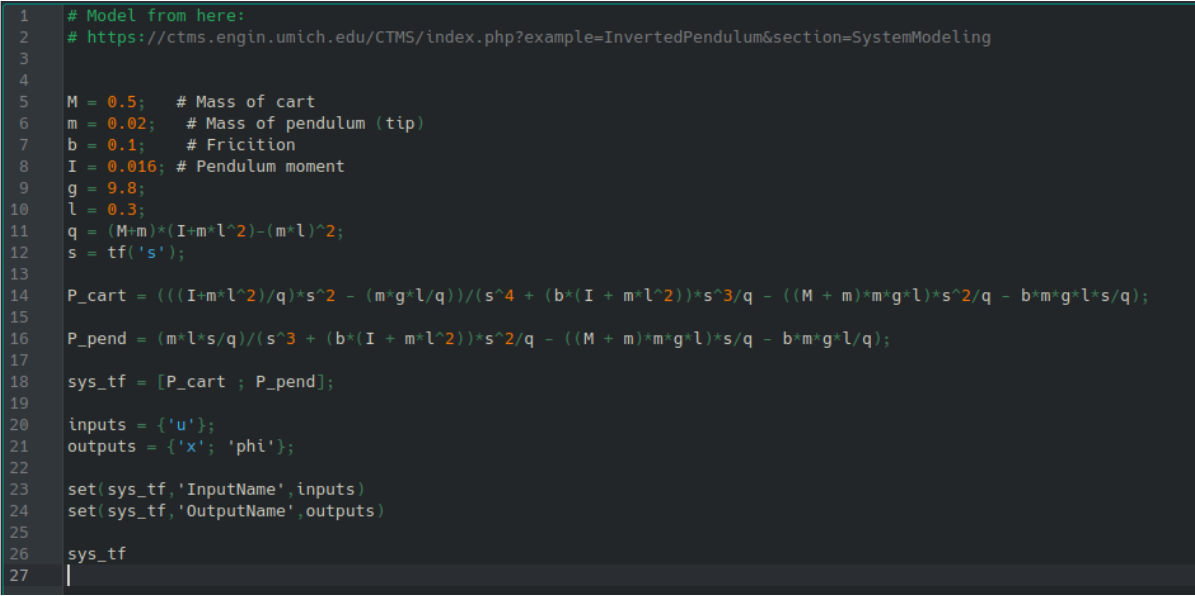
\includegraphics[height=6.5cm]{Calculations}

    Octave math model.
\end{frame}

\begin{frame}
    \frametitle{Calculations (cont.)}

    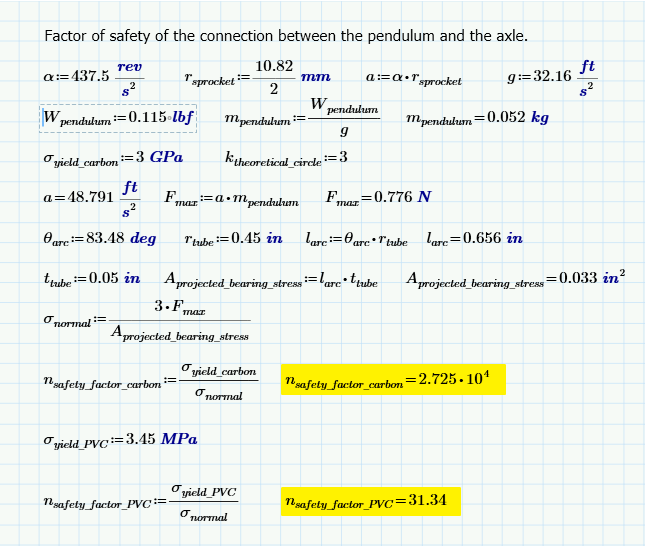
\includegraphics[height=6.5cm]{CalculationsMatt}

    Hand math model.
\end{frame}

\begin{frame}
    \frametitle{Code}

    \begin{columns}
        \begin{column}{0.48\textwidth}
            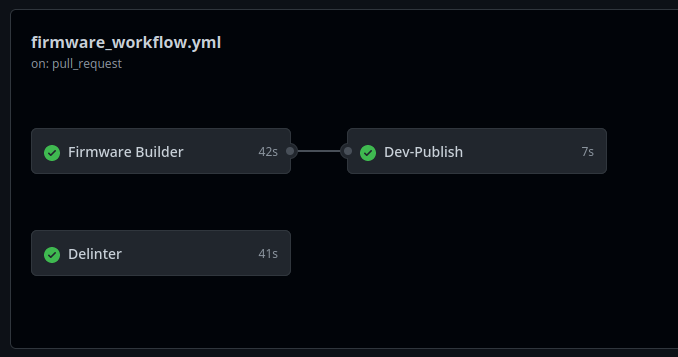
\includegraphics[width=6.5cm]{CodePasses}
        \end{column}

        \begin{column}{0.48\textwidth}
            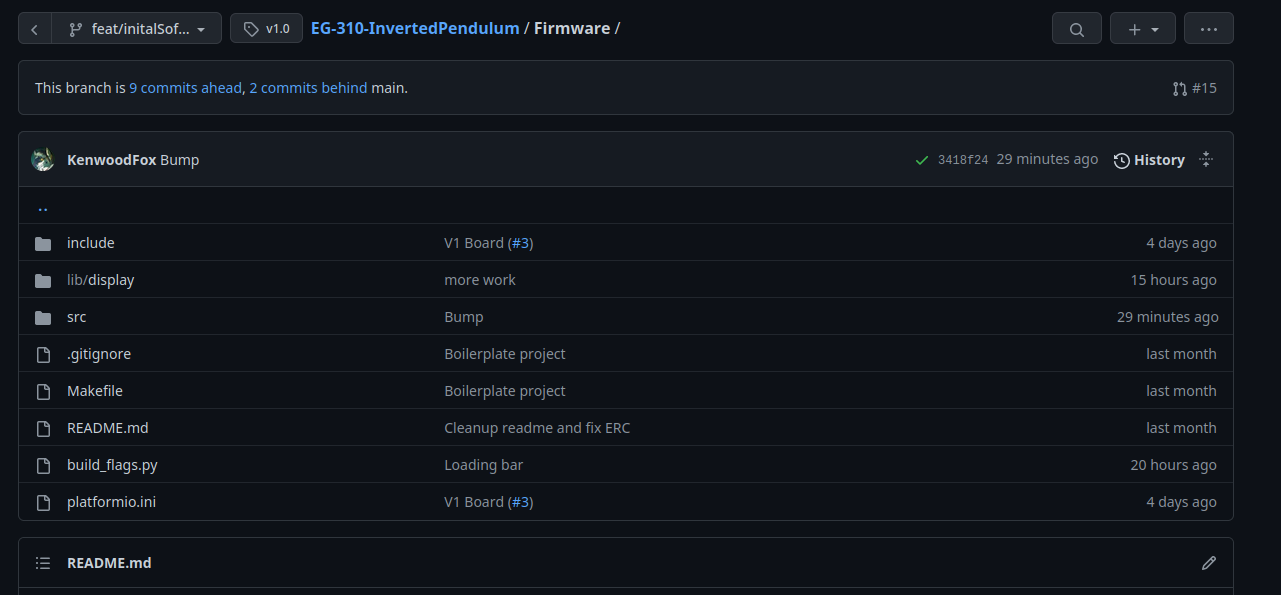
\includegraphics[width=6.5cm]{CodeOnline}
        \end{column}
    \end{columns}
\end{frame}

\begin{frame}
    \frametitle{References}

    
\includegraphics[width=12cm]{CDRReferences}
\end{frame}

\end{document}
